\section{Implementation}
\label{sec:work}
%Efter avsnitten ovan följer nu en beskrivning av vad du gjort. Du ska inte använda rubriken ovan, utan ersätta den med lämpliga rubriker, beroende på ditt arbete. Strukturen ska göras tydlig genom avsnittsrubrikerna. Det är viktigt med en klar och tydlig logisk struktur och ett berättande flöde. Du ska ha med avancerad bakgrundskunskap som är nödvändig för att förstå hur du löst uppgiften, och definiera hypoteser och viktiga begrepp. Beskrivning av experiment ska vara sådan att det ska gå att upprepa experimenten. Om en sådan beskrivning blir väldigt lång och detaljerad kan du lägga den i en bilaga, se nedan.

In this research the code was implemented using Python due to its vibrant echo system of predefined packages already available in its package database.
The over all implementation is described in figure\ref{fig:project_overview} that describes how users annotates the data taken from images on the subject in the scene and how that leads to the results given in\ref{sec:results}.
As can be observed the system is implemented  as a "one shot" static implementation that first collects images in an prepossessing step.
On that database of images the information on what kind of corners there are in each image.


\begin{figure}[ht]
\begin{center}
    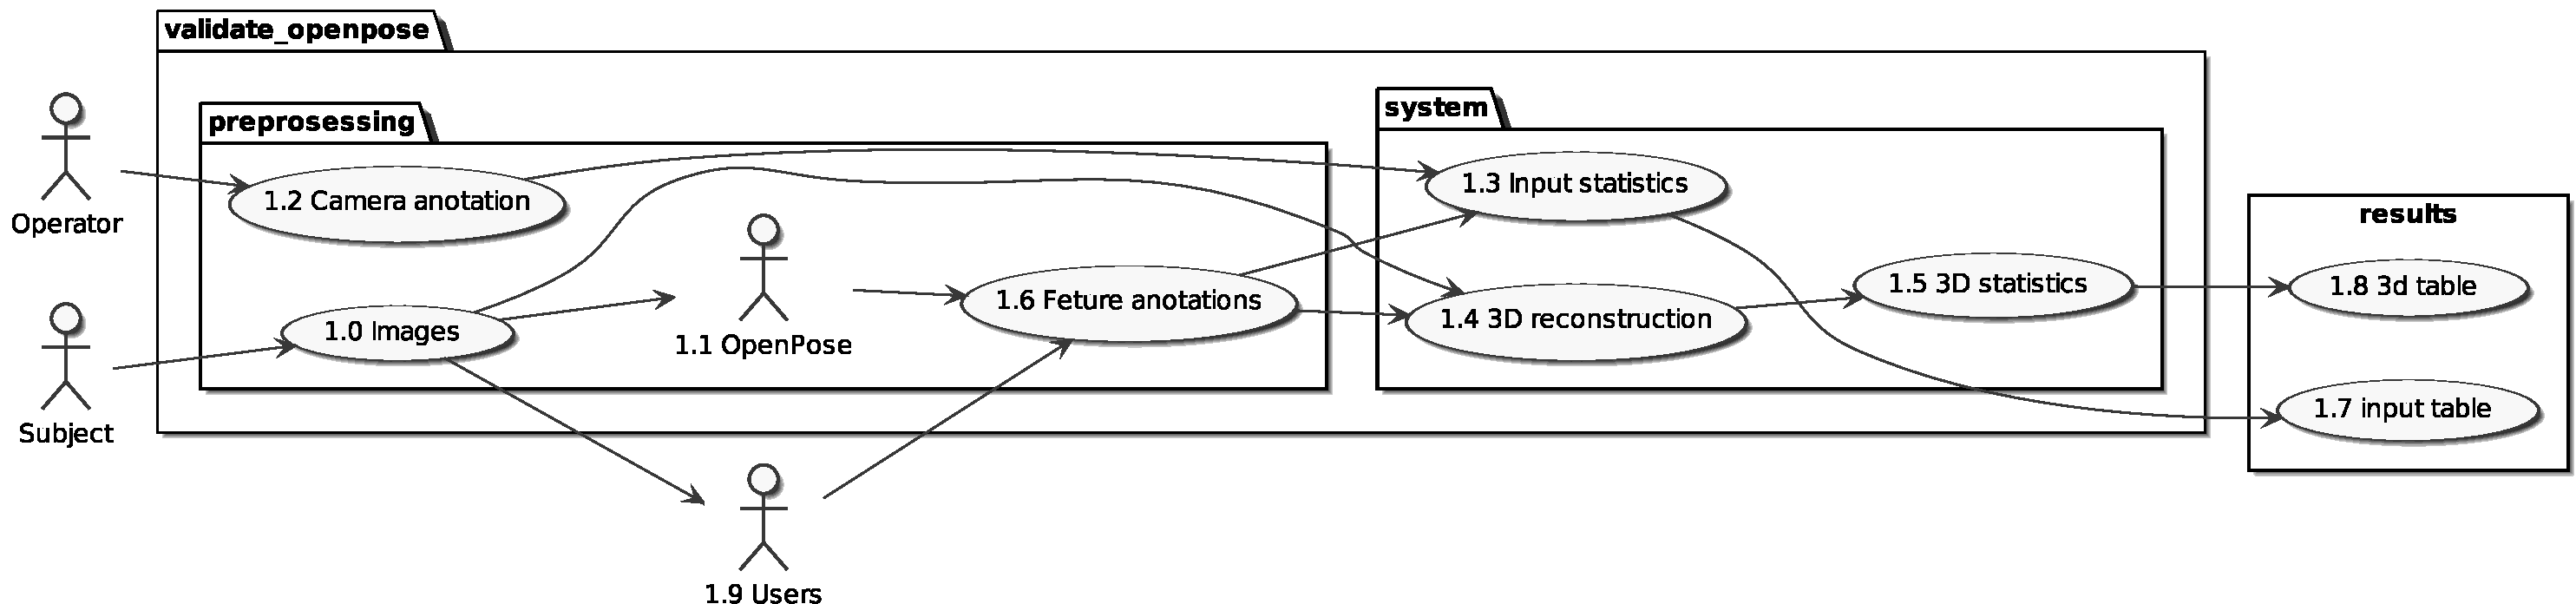
\includegraphics[width=0.9\textwidth]{figures/project_overview.png}
\end{center}
\caption{In this figure the overall intended implementation of the system. The subject is the person on the floor while users are the one who annotates the images. The general camera quadrant where the camera was located is annotated by the Operator who took the images. In this image \openpose is displayed as a human but that is only for clarity that the images are supposed to be annotated equally by both user and \openpose. 1.0 images are stored on the computers file system and can be accessed using Python.}
\label{fig:project_overview}
\end{figure}

Figure~\ref{fig:1.1.openpose_anotation} shows how \openpose works with the system to create the annotations for the features in the image and how it is saved to disk as a \ac{csv} file.
The figure~\ref{fig:1.6.feoture_antotation} shows how that data saved in multiple \ac{csv} files are combined in to one database accessible from a class based \ac{api}
This \ac{api} can be used find relations between users and \openpose or even camera directions.

\begin{figure}[ht]
\begin{center}
    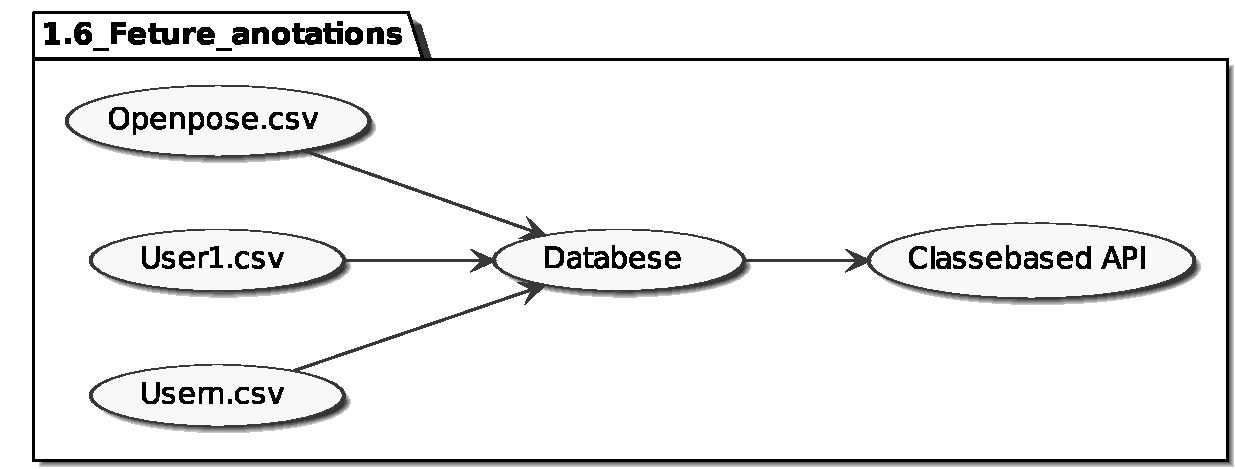
\includegraphics[width=0.3\textwidth]{figures/feature_anotation.png}
\end{center}
\caption{In figure~\ref{fig:project_overview} the block 1.6 Feature Annotations to from \ac{csv} build a database and create an class based API that then 1.3 and 1.4 then uses to future create the validation system. Note that \openpos is only one entity while there are n many users}
\label{fig:1.6.feoture_antotation}
\end{figure}



\begin{figure}[ht]
\begin{center}
    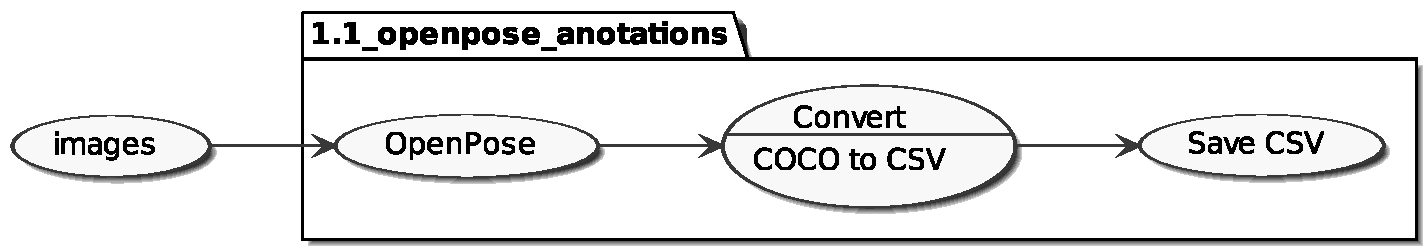
\includegraphics[scale=0.4]{figures/openpose_anotation.png}
\end{center}
\caption{In this figure the implemented step of 1.1 in figure\ref{fig:project_overview} shows how \openpose takes in images and convert annotate, convert and save the annotations as a CSV file.}
\label{fig:1.1.openpose_anotation}
\end{figure}

The figure~\ref{fig:1.3_input_statistics} shows how the input from both the camera quadrant annotation and features is annotated.
Of specific interests is 1.3.6 and 1.3.7 they splits the data into multiple tables that for example 1.3.7 returns for tables, one for each quadrant north, east, south and west.
1.3.4 (a,b) uses equation\ref{eq:impl:muerror} to calculate the median error for that feature with regards to the median of the user group.



\begin{figure}
\begin{center}
    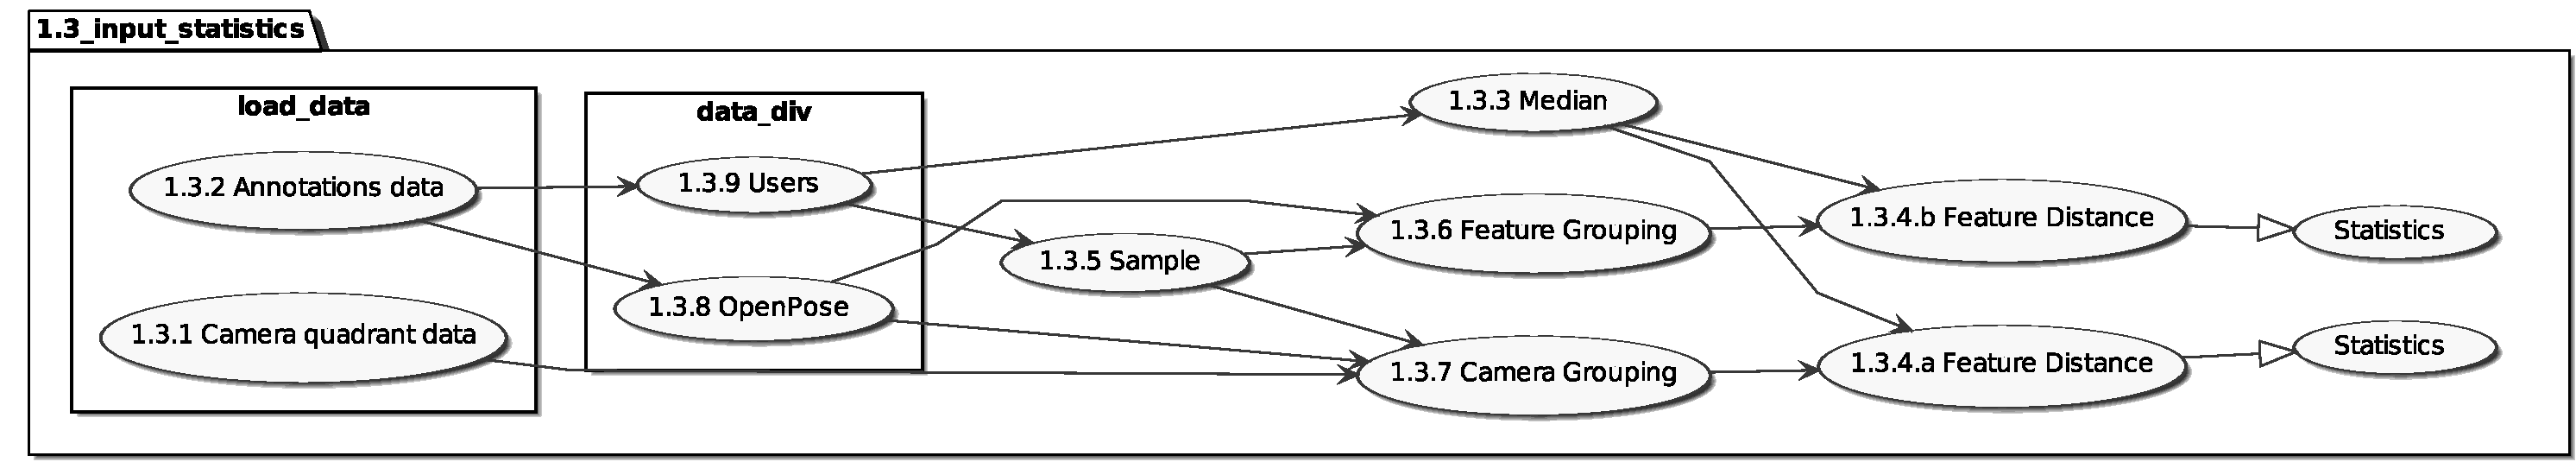
\includegraphics[scale=0.3]{figures/input_statistics.png}
\end{center}
\caption{From block 1.3 in figure~\ref{fig:project_overview}, This figure shows how the input data is processed 1.3.2 loads the annotated data while 1.3.8 and 1.3.9 splits the data up in \openpose and users. 1.3.5 a sample is drawn and the rest of the data makes the 1.3.3 median. 1.3.6 Feature grouping is organising the data according to its features while 1.3.7 organises the data according to Camera quadrant. In 1.3.4 (a,b) the distance equation~\ref{eq:impl:muerror} to calculate the distance from annotated data.}
\label{fig:1.3_input_statistics}
\end{figure}

\begin{figure}
\begin{center}
    \includegraphics[scale=0.26]{../figures/3D_reconstrution.png}
\end{center}
\caption{In thins figure the general function for 3D reconstruction is presented. 1.4.1 Load the camera 3D position and how that works is presented in figure\ref{fig:1.4.1_camerapose}. 1.4.2 loads the features for the 2D features on each image. 1.4.3 represents the majority of the human answers while 1.4.4 Is the minority sample. 1.4.5 is the \openpose feature response. 1.4.6 (o,h and s) is the projective geometry deeper explained in figure~\ref{fig:1.4.6.proj_geometry}. 1.4.8 creates a median $\mu$ constructed form the 3D point cloud in 1.4.6.h. 1.4.9 and 1.4.10 Calculates the distance from the median generated in 1.4.8 and the results are sent to the statistics module~\ref{} }
\label{fig:1.4.3D_reconstrution}
\end{figure}

\begin{figure}
\begin{center}
    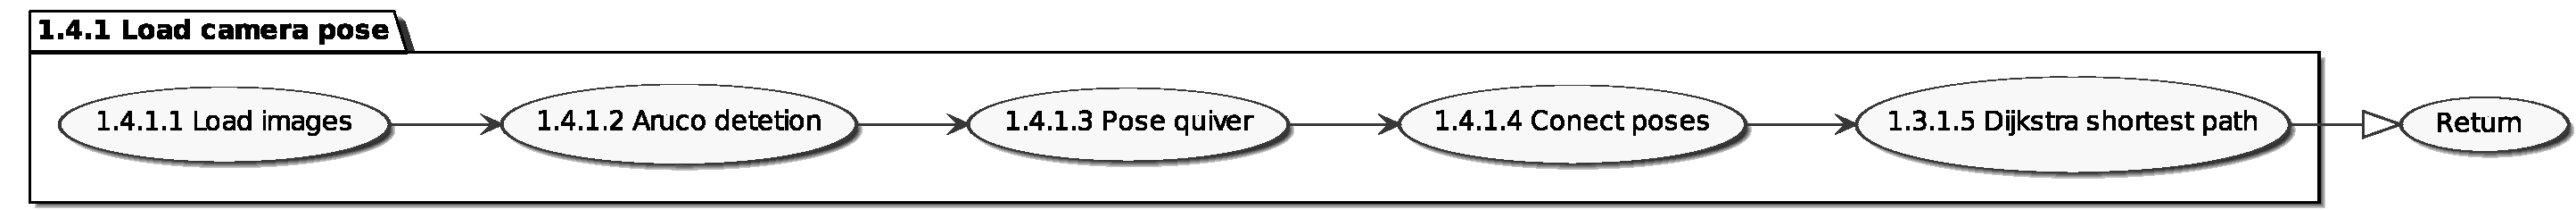
\includegraphics[scale=0.3]{../figures/camerapose.png}
\end{center}
\caption{From figure~\ref{fig:1.4.3D_reconstrution} the position of the camera is calculated in the following steps. 1.4.1.1 Loads the images from the database, 1.4.1.2 Aruco detection detects each individual \aruco in each image and provides the transfer matrix from the camera to the \aruco corner. In 1.4.1.3 the pose quiver connects each corner to each corner in each image figure~\ref{fig:trans_calc} shows the process for that a bit deeper. 1.4.1.4 connect the corner to each corner using the algorithms in~\ref{sub:implement:relative}. 1.4.1.5 Dijkstra is used to derive shortest path from each corner to corner and corner to camera with the position of each step saved in each corner/camera}
\label{fig:1.4.1_camerapose}
\end{figure}


\begin{figure}
\begin{center}
    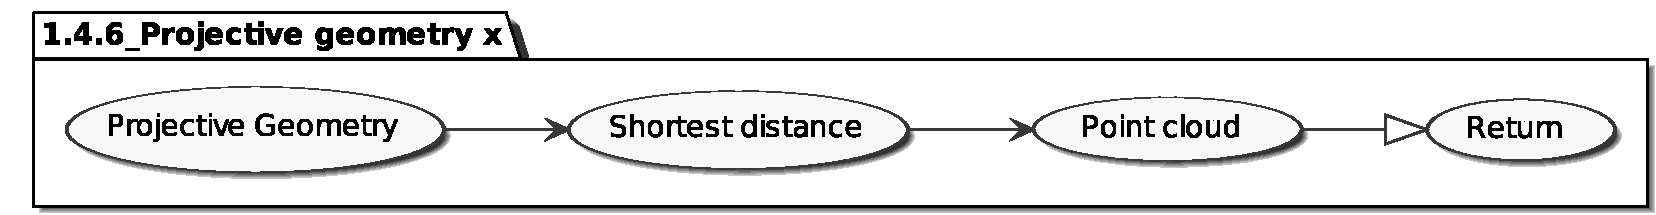
\includegraphics[scale=0.35]{../figures/proj_geometry.png}
\end{center}
\caption{The projective geometry in figure~\ref{fig:1.4.3D_reconstrution} 1.4.6 (o,h and s) is shown in this figure how first the node projective geometry using the calculations in~\ref{sub:Midpoint} to calculate the projective line out of the camera through a feature from ether \openpose or a human. Shortest distance is the distance between ether two ore more lines for each image and each feature, visually demonstrated in figure~\ref{fig:3Dhuman}. This generates a point cloud with point for each shortest distance.}
\label{fig:1.4.6.proj_geometry}
\end{figure}







Those corners are then identified and connected souch that the corner nr 1 in image 1 is connected to corner nr 1 in image 2.
This process builds a pose quiver how each corner is connected to each image.
With that process done the \aruco{ } library can generate the $\vec{t}$ and $\vec{r}$ that determines the camera in relation to that corner.

However, its not as explained in\ref{sub:implement:relativepath} the reference that is interesting.
Instead the pose quiver is used to calculate the path from origin to the camera using transfer matrices.
% This is done by using Dijkstras algorithm for the shortest path and then the algorithm~\ref{alg:inverse},~\ref{alg:relative}
%On the implementation side this is done by first calculating the path from the origin to the camera using Dijkstras algorithm.

On the implementation side the first step in the code is calculating the cumulative transfer matrix from origin to each corner by first setting the origin as $I$.

\input{figures/trans_calc.latex}


